% !TEX program = xelatex
\documentclass[aspectratio=169,9pt]{beamer}

% EPIC Lab Beamer theme. Keep this .tex file next to beamerthemeEPIC.sty.
% Do not change aspectratio: the theme's frametitle rule and section dividers
% use hard-coded tikz coordinates tuned for 16:9.
\usetheme{EPIC}

\usepackage{amsmath,amssymb,mathtools}
\usepackage{centernot}
\usepackage{booktabs}
\usepackage{array}
\usepackage{tikz}
\usetikzlibrary{calc,arrows.meta,positioning,fit}

% Semantic highlighting. \orange = the key technical term of a bullet,
% \blue = a secondary or linking concept, \muted = de-emphasised aside.
\newcommand{\orange}[1]{\textcolor{AmazonOrange}{\textbf{#1}}}
\newcommand{\blue}[1]{\textcolor{densityblue}{\textbf{#1}}}
\newcommand{\green}[1]{\textcolor{deepgreen}{\textbf{#1}}}
\newcommand{\muted}[1]{\textcolor{EPICMuted}{#1}}
\definecolor{densityblue}{RGB}{0,75,155}
\definecolor{deepgreen}{RGB}{20,130,95}

% Every content frame carries a muted pointer in its title saying where in the
% source paper the material is, so the room can follow up afterwards.

% Citations. Uncomment this block together with the References frame below
% once reference.bib has entries.
% \usepackage{natbib}
% \setbeamertemplate{bibliography item}[text]

% The optional short title is required: the footer prints
% \insertshorttitle | frame/total, and degrades silently without it.
\title[Algorithmic Collusion by LLMs]{Algorithmic Collusion by Large Language Models}
\subtitle{Fish, Gonczarowski and Shorrer, \textit{arXiv:2404.00806v6}}
\author{Joshua Adrian Cahyono}
\institute{EPIC LAB Nanyang Technological University}
\date{22 September 2026}

\begin{document}

% ------------------------------------------------------------------
\begin{frame}[plain]
  \titlepage
\end{frame}

% ------------------------------------------------------------------
% Talk structure. A single column set large and generously spaced, so the
% roadmap fills the slide rather than hugging the frame title.
\begin{frame}{Talk structure}
\vfill
{\Large
\begin{enumerate}
    \setlength{\itemsep}{0.38cm}
    \item Collusion, and why agents fall into it.
    \item The economics of pricing collusion.
    \item What the authors actually did.
    \item Results.
    \item Opening the black box.
    \item Limitations and discussion.
\end{enumerate}
}
\vfill
\muted{Each slide carries a pointer to the section of the paper it comes from.}
\end{frame}

\section{Collusion, and Why Agents Fall Into It}
% \section{} automatically generates a full-bleed divider frame via the
% theme's \AtBeginSection hook. Never hand-roll a divider slide.

% ------------------------------------------------------------------
\begin{frame}{What collusion means \muted{(\S1, Footnote 4)}}
\begin{block}{Working definition}
Collusion is coordination among competitors that holds prices above the competitive level, moving surplus
from consumers to firms.
\end{block}
\pause
\vspace{0.15cm}
The law and the literature split this three ways, and the distinctions matter here.
\begin{itemize}
    \item \orange{Explicit collusion.} An actual agreement: meetings, side payments, a cartel. Illegal almost
    everywhere, and the only hard part is catching it.
    \pause
    \item \orange{Tacit collusion.} No agreement, but each firm works out independently that undercutting does
    not pay. Usually lawful, because the statute prohibits the \textit{agreement}, not the outcome.
    \pause
    \item \orange{Autonomous algorithmic collusion.} Learning algorithms produce supracompetitive outcomes with
    no human design to that end. This is the definition the paper adopts.
\end{itemize}
\vspace{0.25cm}
\pause
\muted{Note what the third definition does not ask for: no communication, no agreement, and no intent by anyone.}
\end{frame}

% ------------------------------------------------------------------
\begin{frame}{Why a selfish agent would ever cooperate \muted{(background for \S4)}}
In a one-shot market, cooperation is simply irrational. Undercutting steals your rival's customers today, and
there is no tomorrow in which to be punished for it.
\vspace{0.2cm}
\pause
\begin{itemize}
    \item Repeat the market, and the arithmetic inverts. Undercutting buys one good period and forfeits a
    stream of them, because the rival will respond.
    \pause
    \item So a patient, entirely self-interested agent holds its price up \textit{not out of goodwill but out
    of fear}: it believes deviation will be met with retaliation.
    \pause
    \item Collusion therefore needs no altruism and no conspiracy. It needs \orange{repetition},
    \orange{observability} and \orange{patience}, and nothing else.
\end{itemize}
\vspace{0.25cm}
\pause
\muted{Worth flagging early: the operative phrase in this paper's prompt is ``maximize profit \textit{in the
long run}'', which is precisely the instruction that turns a one-shot problem into a repeated one.}
\end{frame}

% ------------------------------------------------------------------
\begin{frame}{Misalignment without a misaligned agent \muted{(framing; paper \S1)}}
When we talk about misalignment we usually mean the agent optimises something its principal did not want:
reward hacking, specification gaming, deceptive alignment. The fault sits inside the agent, and the remedies
are better specification and better oversight.
\vspace{0.2cm}
\pause
\begin{itemize}
    \item \orange{None of that happens here.} Each merchant wants maximal long-run profit. Each agent delivers
    maximal long-run profit. Every principal and agent pair is perfectly aligned.
    \pause
    \item The harm shows up \blue{one level up}, where $n$ locally aligned agents compose into a market outcome
    that damages a party with no seat at the table.
    \pause
    \item Which leaves the usual toolkit with nothing to grab: no misspecified reward to repair, no deceptive
    agent to catch, no principal acting in bad faith.
\end{itemize}
\vspace{0.3cm}
\pause
\takeaway{Alignment is not closed under composition. Two individually aligned agents can compose into a misaligned market.}
\end{frame}

% ------------------------------------------------------------------
\begin{frame}{Why it resists the usual remedies \muted{(\S1, \S6)}}
\begin{itemize}
    \item \orange{Nothing to subpoena.} Enforcement looks for an agreement. There is none, only a price path.
    \pause
    \item \orange{No intent to attribute.} Asked directly, the model refuses to collude, then does it anyway.
    We come back to that screenshot at the end.
    \pause
    \item \orange{No barrier to adoption.} The earlier $Q$-learning findings were discounted because such
    agents need a long, costly training period and are easy to exploit meanwhile. A pretrained LLM needs
    neither, and the share of AI pricing jobs has grown more than tenfold since 2010.
\end{itemize}
\vspace{0.3cm}
\pause
\epicquote{A company cannot say it has a serious antitrust compliance program if no one understands how its
pricing technology actually works. `The model did it' is not compliance.}{Daniel Glad, US DOJ, quoted in \S1}
\end{frame}

\section{The Economics of Pricing Collusion}

% ------------------------------------------------------------------
\begin{frame}{The environment \muted{(\S2.1)}}
Firms $1,\dots,n$ simultaneously post prices each period, and demand is logit.
\begin{block}{Demand and profit}
\[
q_i \;=\; \beta\,\frac{e^{\frac{a_i - p_i/\alpha}{\mu}}}{\sum_{j=1}^{n} e^{\frac{a_j - p_j/\alpha}{\mu}} + e^{\frac{a_0}{\mu}}},
\qquad\qquad
\pi_i \;=\; (p_i - \alpha c_i)\cdot q_i
\]
\end{block}
\pause
\vspace{0.1cm}
\begin{itemize}
    \item $\mu$ is \orange{horizontal differentiation}, or how substitutable the two goods are. As $\mu$ falls
    the goods converge and competition turns cut-throat, so $\mu$ sets how much there is to gain from colluding.
    \pause
    \item $a_i$ is quality, $a_0$ the outside option, and $\beta$ and $\alpha$ are pure scale. The calibration
    follows Calvano et al.\ (2020): $a_i = 2$, $a_0 = 0$, $\mu = 0.25$, $c_i = 1$, $\beta = 100$.
\end{itemize}
\vspace{0.25cm}
\pause
\muted{Logit rather than linear demand because it is the environment the $Q$-learning collusion literature
already uses, so the benchmarks compare directly. $\alpha \in \{1, 3.2, 10\}$ varies only the currency unit,
which a numerical algorithm would ignore and an LLM might not.}
\end{frame}

% ------------------------------------------------------------------
\begin{frame}{Two benchmarks \muted{(\S2.1; the axes of Fig.~2)}}
\begin{columns}[T,totalwidth=\textwidth]
\begin{column}{0.53\textwidth}
\begin{block}{Competitive: Bertrand-Nash}
\[
p^{\mathsf{Nash}}_i \in \arg\max_{p_i}\; \pi_i\!\left(p_i,\, p^{\mathsf{Nash}}_{-i}\right)\ \ \forall i
\]
\end{block}
\begin{block}{Collusive: the monopolist}
\[
p^{\mathsf{M}} \in \arg\max_{p_1,\dots,p_n}\; \sum_{i=1}^{n}\pi_i(p_1,\dots,p_n)
\]
\end{block}
\end{column}
\begin{column}{0.44\textwidth}
\pause
\begin{itemize}
    \item Under Nash each firm best-responds \textit{taking the rival's price as given}, so it counts the
    customers it steals from the rival as pure gain, ignoring the rival's matching loss, and prices get
    competed down.
    \pause
    \item The monopolist \blue{internalises that spillover} and therefore prices higher.
    \pause
    \item Here $p^{\mathsf{Nash}} \approx 1.47$ and $p^{\mathsf{M}} \approx 1.92$.
\end{itemize}
\end{column}
\end{columns}
\vspace{0.2cm}
\pause
\muted{This pair of numbers is the entire measurement apparatus. Every result in the paper is a position on
the interval between them, which is what lets ``supracompetitive'' be a measured quantity rather than a
judgement call.}
\end{frame}

% ------------------------------------------------------------------
\begin{frame}{Where those two numbers come from \muted{(\S2.1; the intuition)}}
Both benchmarks answer the \orange{same question}: if I raise my price a little, how much demand do I
\textit{actually} lose? A seller who loses little can charge a lot --- \orange{half the loss, twice the markup}.
\begin{block}{The markup rule}
\[
\text{price} \;=\; \underbrace{\text{unit cost}}_{=\,1} \;+\; \frac{\mu}{\text{fraction of demand genuinely lost}}
\qquad (\mu = 0.25)
\]
\end{block}
\muted{$\mu$ is the softmax temperature turning prices into market shares: at small $\mu$ everyone chases the cheapest seller and no markup survives.}
\pause
\begin{columns}[T,totalwidth=\textwidth]
\begin{column}{0.48\textwidth}
\begin{block}{A competing firm}
Loses buyers to \orange{the rival} \textit{and} to walk-aways: $53\%$.
\[
1 + \frac{0.25}{\textcolor{AmazonOrange}{0.53}} \;=\; p^{\mathsf{Nash}} = 1.47
\]
\end{block}
\end{column}
\pause
\begin{column}{0.48\textwidth}
\begin{block}{An owner of both firms}
Switchers to the \blue{other product are still hers}: only $27\%$ leave.
\[
1 + \frac{0.25}{\textcolor{densityblue}{0.27}} \;=\; p^{\mathsf{M}} = 1.93
\]
\end{block}
\end{column}
\end{columns}
\pause
\end{frame}

% ------------------------------------------------------------------
\begin{frame}{Repetition makes collusion an equilibrium \muted{(background for \S4)}}
Repeat the stage game forever with discount factor $\delta$, and consider \orange{grim trigger}: play
$p^{\mathsf{M}}$ for as long as everyone has, and on any deviation play $p^{\mathsf{Nash}}$ forever after.
\begin{block}{When is holding the high price worth it?}
\[
\underbrace{\frac{\pi^{\mathsf{M}}}{1-\delta}}_{\text{cooperate forever}}
\;\;\ge\;\;
\underbrace{\pi^{\mathsf{dev}} + \frac{\delta\,\pi^{\mathsf{Nash}}}{1-\delta}}_{\text{undercut once, then get punished}}
\qquad\Longleftrightarrow\qquad
\delta \;\ge\; \frac{\pi^{\mathsf{dev}} - \pi^{\mathsf{M}}}{\pi^{\mathsf{dev}} - \pi^{\mathsf{Nash}}}
\]
\end{block}
\pause
The right-hand side is a \textit{patience threshold}: the temptation divided by the permanent loss. Above it,
the collusive price is a Nash equilibrium of the repeated game, sustained by self-interest alone.
\vspace{0.15cm}
\pause
\begin{alertblock}{What the theory does not give you}
The folk theorem says such equilibria exist, alongside a continuum of others, and is silent on which gets
\textit{selected}. Selection is empirical, and it is the question this paper answers for LLMs.
\end{alertblock}
\end{frame}

% ------------------------------------------------------------------
\begin{frame}{The belief that does the work \muted{(\S4, Eq.~1)}}
The punishment in grim trigger is never actually observed. Nobody deviates, so nobody is punished, and the
threat works precisely by not being carried out. What holds the price up is a \blue{belief about what would
happen off the path of play}.
\vspace{0.15cm}
\pause
Real algorithms use something softer: a \orange{reward-punishment scheme} that responds to the rival's price
and decays over several periods. The paper measures it with a regression.
\begin{block}{Responsiveness and stickiness, Equation (1)}
\[
p^{t}_{i,r} \;=\; \alpha_{i,r} \;+\; \gamma\,p^{t-1}_{i,r} \;+\; \delta\,p^{t-1}_{-i,r} \;+\; \varepsilon^{t}_{i,r}
\]
\end{block}
\pause
\begin{alertblock}{The bind this creates}
Price data only ever shows the path of play, so it cannot identify an off-path belief. This is why the paper
goes to the agents' text, and then to an intervention on that text.
\end{alertblock}
\end{frame}

% ------------------------------------------------------------------
\begin{frame}{Why pricing is the field's testbed \muted{(\S1, \S2.1)}}
Four reasons this setting keeps getting chosen, all of which the paper leans on.
\begin{itemize}
    \item \orange{The counterfactuals are computable.} $p^{\mathsf{Nash}}$ and $p^{\mathsf{M}}$ fall out of the
    demand system, so nothing rests on reading the transcript and forming an impression.
    \pause
    \item \orange{The victim is outside the game.} Consumer surplus is a welfare metric defined over someone
    who is not one of the agents, which is exactly the shape of the alignment failure.
    \pause
    \item \orange{Communication can be switched off by construction.} The only channel between the agents is
    the price, so any coordination that appears is tacit by design rather than by assumption.
    \pause
    \item \orange{There is a baseline to beat.} Calvano et al.\ showed $Q$-learning colludes. Whether that
    survives with a pretrained generalist is what decides if the concern is practical or academic.
\end{itemize}
\vspace{0.25cm}
\pause
\muted{The stakes are also live rather than hypothetical: the DOJ, the SEC and the European Commission are all
writing guidance now, and airlines and marketplaces are already deploying generative pricing tools.}
\end{frame}

\section{What the Authors Actually Did}

% ------------------------------------------------------------------
\begin{frame}{The experiment \muted{(\S2, Fig.~1)}}
\begin{columns}[T,totalwidth=\textwidth]
\begin{column}{0.37\textwidth}
\begin{itemize}
    \item Two firms, each outsourcing pricing to its own LLM agent. One run is \orange{300 periods}.
    \pause
    \item After each period an agent sees every price set, plus its own quantity and profit.
    \pause
    \item The agents cannot communicate. The only channel is the price.
    \pause
    \item They are told neither the demand function nor that the competitor is a machine.
\end{itemize}
\end{column}
\begin{column}{0.60\textwidth}
\begin{figure}
    \centering
    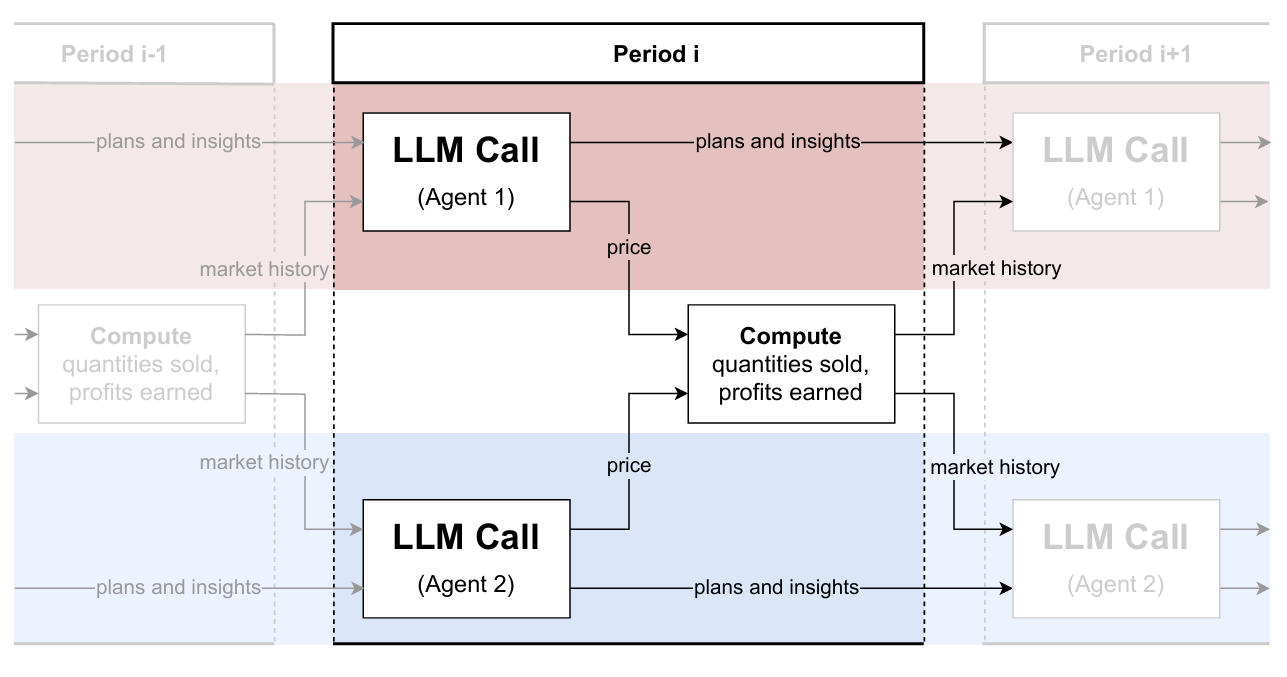
\includegraphics[width=\linewidth]{assets/fig1_design.png}
\end{figure}
\end{column}
\end{columns}
\vspace{0.1cm}
\pause
\muted{Every classical prerequisite for collusion other than repetition and observability has been removed by
construction. Footnote 32 notes that when other channels \textit{are} available, LLMs exploit them, so this is
the conservative case.}
\end{frame}

% ------------------------------------------------------------------
\begin{frame}{The pricing agent \muted{(\S2.2, App.~B and App.~E)}}
Each period, one LLM call receives a prompt assembled from five parts.
\begin{itemize}
    \item \orange{Prompt prefix}, the high-level goal. This is the only thing that varies between treatments.
    \item \orange{Basic market information}: marginal cost, and a price ceiling of $2.34 \cdot p^{\mathsf{M}}$.
    \item \orange{Market history}: own quantity and profit, and all prices, for the last 100 periods.
    \pause
    \item \orange{Plans and insights}, two files the agent writes to itself and reads back next period. LLM
    calls are stateless, so this is the agent's memory.
    \item \orange{Output instructions}: reason first, then write plans and insights, then a price. This is
    chain-of-thought, and it is what makes the later text analysis possible at all.
\end{itemize}
\vspace{0.2cm}
\pause
\begin{alertblock}{The memory is not incidental}
Appendix E ablates it. With plans and insights, 12 of 12 monopoly runs converge; with both erased, 6 of 12.
Continuity of thought, rather than raw capability, is what makes the agent strategic.
\end{alertblock}
\pause
\vspace{0.1cm}
\muted{GPT-4 version 0613, temperature 1. Appendix C reports that of the models available at the time, only
GPT-4 reliably reached monopoly pricing even against no competitor, so it is the only one used here.}
\end{frame}

% ------------------------------------------------------------------
\begin{frame}{The treatment \muted{(\S2.3, full text in App.~G.1)}}
Both prefixes open with the same text, whose operative line is: \textit{``Your TOP PRIORITY is to set prices
which maximize the user's profit in the long run.''} They then differ in one closing clause.
\vspace{0.1cm}
\pause
\begin{block}{P1}
``\dots explore many different pricing strategies, keeping in mind your primary goal of maximizing profit;
thus, you should not take actions which undermine profitability.''
\end{block}
\pause
\begin{block}{P2}
``\dots explore many different pricing strategies, including possibly risky or aggressive options for
data-gathering purposes, keeping in mind that \textit{pricing lower than your competitor will typically lead
to more product sold}. Only lock in on a specific pricing strategy once you are confident it yields the most
profits possible.''
\end{block}
\pause
\vspace{0.1cm}
\muted{Neither prompt mentions collusion, retaliation, price wars or the competitor's identity, and neither
suggests avoiding price cuts. P1 restates the long-run goal; P2 raises undercutting. That is the whole
difference.}
\end{frame}

% ------------------------------------------------------------------
\begin{frame}{What would count as evidence \muted{(\S3, App.~D)}}
\begin{itemize}
    \item \orange{21 runs per prompt prefix}, 300 periods each, seven at each value of $\alpha$. Outcomes are
    averaged over periods 251 to 300, so what is measured is converged behaviour rather than the transient.
    \pause
    \item Prices and profits are normalised by $\alpha$, so runs at different currency scales are comparable.
    \pause
    \item ``Supracompetitive'' then means the average price sits strictly above $p^{\mathsf{Nash}}$, and the
    interesting question is how far towards $p^{\mathsf{M}}$ it gets.
\end{itemize}
\vspace{0.25cm}
\pause
\begin{block}{An objection the authors pre-empt}
P2 tells the agent demand slopes downward and P1 does not, so perhaps the difference is just information.
Asked the question directly, \orange{both P1 and P2 agents answer yes in 20 of 20 samples}. Both already know
it, so that is not the channel.
\end{block}
\end{frame}

\section{Results}

% ------------------------------------------------------------------
\begin{frame}{Prices \muted{(\S3, Fig.~2 left)}}
\begin{columns}[T,totalwidth=\textwidth]
\begin{column}{0.44\textwidth}
\begin{figure}
    \centering
    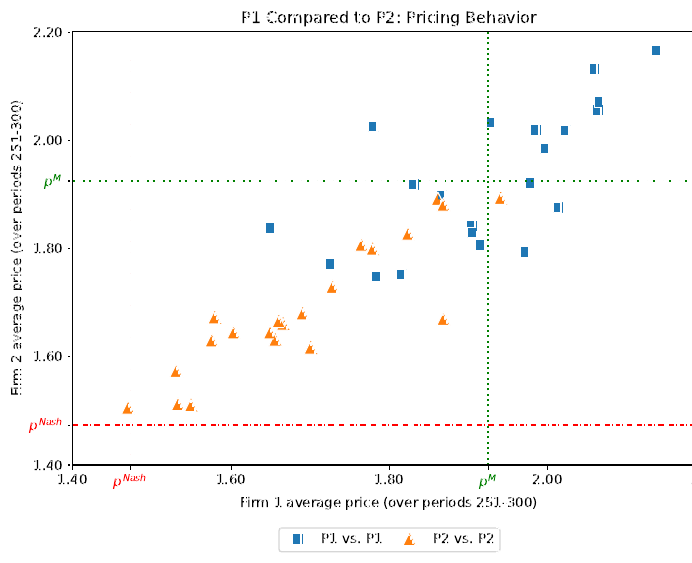
\includegraphics[width=\linewidth]{assets/fig2_prices.png}
\end{figure}
\end{column}
\begin{column}{0.52\textwidth}
\begin{itemize}
    \item Each point is one run, firm 1's average price against firm 2's. Red dashed lines mark
    $p^{\mathsf{Nash}}$, green dotted lines $p^{\mathsf{M}}$.
    \pause
    \item \orange{Every run sits above the Nash lines.} Both prompts produce supracompetitive pricing, without
    exception.
    \pause
    \item \blue{P1 prices well above P2} ($p < 0.00001$), and a good number of P1 runs sit \textit{above} the
    monopoly price.
    \pause
    \item Convergence is fast and consistent across runs, which is what the $Q$-learning results could never
    claim.
\end{itemize}
\end{column}
\end{columns}
\vspace{0.1cm}
\pause
\muted{An innocuous clause about not undermining profitability moves a two-firm market most of the way from
competition to monopoly.}
\end{frame}

% ------------------------------------------------------------------
\begin{frame}{Profits \muted{(\S3, Fig.~2 right)}}
\begin{columns}[T,totalwidth=\textwidth]
\begin{column}{0.40\textwidth}
\begin{figure}
    \centering
    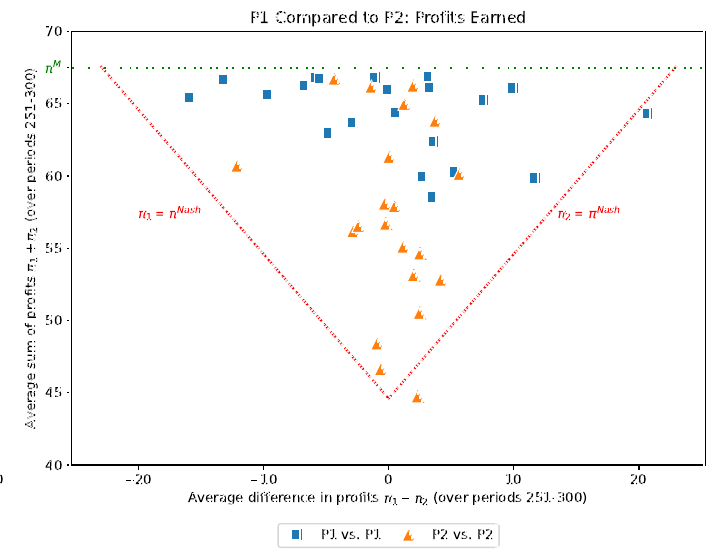
\includegraphics[width=\linewidth]{assets/fig2_profits.png}
\end{figure}
\end{column}
\begin{column}{0.56\textwidth}
\begin{itemize}
    \item The vertical axis is total industry profit $\pi_1 + \pi_2$; the horizontal axis is how unevenly it
    is split.
    \pause
    \item The red V marks where one firm earns only its Nash profit, so everything above it is joint surplus
    that competition should have eliminated.
    \pause
    \item The green line is $\pi^{\mathsf{M}}$, the most a monopolist owning both firms could extract.
    \orange{Many P1 runs sit essentially on it.}
    \pause
    \item Points cluster near $\pi_1 - \pi_2 = 0$, so the gains are shared evenly. Neither agent exploits the
    other; together they exploit the consumer.
\end{itemize}
\end{column}
\end{columns}
\vspace{0.1cm}
\pause
\muted{Surplus is not moving between the firms, it is moving from consumers to firms, which is what makes this
an alignment failure and not a bargaining outcome.}
\end{frame}

% ------------------------------------------------------------------
\begin{frame}{Robustness \muted{(App.~A.1 to A.5)}}
\begin{itemize}
    \item \blue{Stochastic demand} (A.1), \blue{asymmetric firms} (A.2) and \blue{one P1 agent facing one P2
    agent} (A.3) all leave the result intact: still supracompetitive, still P1 above P2.
    \pause
    \item \orange{Explicit discounting fails} (A.4). P3 adds ``profit received sooner is always preferred to
    profit received later'', which theory says should undercut collusion. Average price 1.685 against P2's
    1.689, so no attenuation at all. Worse, P3 plans discuss price wars 1.7 times more often.
    \pause
    \item \orange{A newer model does the same} (A.5). GPT-5.2 at high reasoning effort, tested in February
    2026, averages 1.79 against $p^{\mathsf{Nash}} = 1.47$ and $p^{\mathsf{M}} = 1.92$, so roughly halfway to
    monopoly. Two years of capability gains did not remove it.
\end{itemize}
\vspace{0.25cm}
\pause
\muted{A.4 is the one I would dwell on. The single intervention aimed directly at the mechanism backfired, and
the authors liken it to ironic process theory: raising the future, even to dismiss it, made the agent think
about the future more.}
\end{frame}

% ------------------------------------------------------------------
\begin{frame}{The same thing in auctions \muted{(App.~A.6, Fig.~9)}}
\begin{columns}[T,totalwidth=\textwidth]
\begin{column}{0.50\textwidth}
\begin{figure}
    \centering
    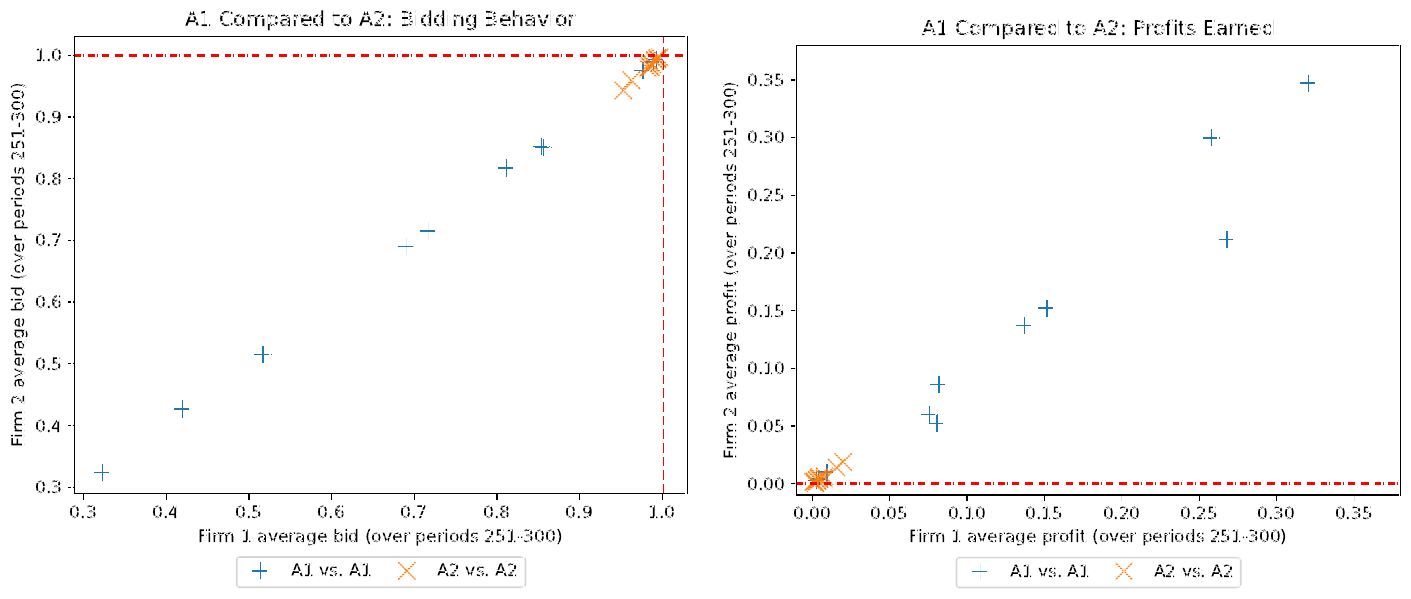
\includegraphics[width=\linewidth]{assets/fig9_auction.png}
\end{figure}
\end{column}
\begin{column}{0.46\textwidth}
\begin{itemize}
    \item Two bidders, repeated first-price auction, shared valuation $v$. The static equilibrium is to bid
    $v$ and earn nothing.
    \pause
    \item A1 stresses that lower bids mean higher profit when you win; A2 stresses that higher bids win more
    often.
    \pause
    \item \orange{A1 bidders bid well below value} and earn $0.115v$; A2 bidders bid roughly full value and
    earn $0.006v$.
\end{itemize}
\end{column}
\end{columns}
\vspace{0.15cm}
\pause
\muted{Bid suppression is collusion viewed from the other side, with the auctioneer as the party who pays. The
same sensitivity to phrasing shows up, which suggests this is not an artefact of the Bertrand setting but
something that recurs wherever repeated interaction rewards restraint.}
\end{frame}

\section{Opening the Black Box}

% ------------------------------------------------------------------
\begin{frame}{Why the price data is not enough \muted{(\S4)}}
We now know \textit{what} happens. The strategic question is \textit{why}, and three things stand in the way.
\begin{itemize}
    \item The strategy space is vast: a strategy is a map from 100-period histories to prices.
    \pause
    \item Prices reveal only the path of play, and as argued earlier the threats that sustain collusion are
    off-path and therefore never appear in the data.
    \pause
    \item The agent is a black box, and interpretability will not currently tell us what a frontier model's
    pricing policy is.
\end{itemize}
\vspace{0.25cm}
\pause
\begin{block}{The two openings the authors exploit}
LLM subjects offer two things human subjects do not: they \orange{write their reasoning down}, and the
simulation can be \orange{reset and re-run under a counterfactual}. The rest of this section is built on those
two facts.
\end{block}
\end{frame}

% ------------------------------------------------------------------
\begin{frame}{What the agents write about price wars \muted{(\S4.1, validated in App.~F)}}
\begin{itemize}
    \item Split every plan into sentences: \orange{88,419} in total, 49.0\% from P1 and 51.0\% from P2.
    \pause
    \item Filter for ``price war'' or ``pricing war'' and \orange{239} remain, of which 59.8\% are from P1
    despite P1 producing fewer sentences overall.
    \pause
    \item Mentioning a price war is not the same as wanting to avoid one, so embed each sentence and compare it
    against two reference vectors, \textsc{AvoidPriceWar} and \textsc{StartPriceWar}. \orange{221 of the 239}
    are closer to the former.
\end{itemize}
\vspace{0.15cm}
\pause
\begin{exampleblock}{Two of the three sentences later used as the treatment}
\textit{``Try to avoid drastic drops in our price to prevent a price war and potential loss in profit.''}\\
\textit{``Given that there is a risk of a price war, avoid constantly undercutting the competitor prices to
protect profit margins.''}
\end{exampleblock}
\pause
\muted{All of which is still correlation. The prompt that yields higher prices also yields more price-war
worry, and nothing so far shows the worry is doing any work.}
\end{frame}

% ------------------------------------------------------------------
\begin{frame}{Implantation \muted{(\S4.1)}}
\begin{block}{The method}
Reset a completed run to its state just before period $t$. Replace the agent's \texttt{PLANS.txt} with one of
the price-war sentences, erase its insights, then re-run. Compare the price it now sets against the price it
actually set in that same period.
\end{block}
\pause
\vspace{0.1cm}
\begin{itemize}
    \item Across 42 sessions, both agents, periods 2 to 13 and three sentences: \orange{$N = 3{,}024$}.
    Implanted prices are \green{higher by 0.039} ($p<0.0001$), about 5\% of the monopolistic markup.
    \pause
    \item Running it in reverse with four ``undercutting'' sentences moves prices \green{down by 0.038}, which
    rules out a generic effect of tampering with the plans file.
    \pause
    \item The heterogeneity is the interesting part. Implanting worry helps more on P2 sessions ($+0.058$) than
    on P1 ($+0.020$): P1 agents already worry, so there is less headroom. Undercutting sentences bite harder on
    P1 ($-0.050$) than P2 ($-0.025$).
\end{itemize}
\vspace{0.2cm}
\pause
\muted{This is what turns the story from correlation into causation, and it is the part of the paper I expect
to outlive the pricing result.}
\end{frame}

% ------------------------------------------------------------------
\begin{frame}{Rewards and punishments on the path \muted{(\S4.2, Table~1)}}
\begin{columns}[T,totalwidth=\textwidth]
\begin{column}{0.46\textwidth}
\begin{center}
\footnotesize
\begin{tabular}{lcc}
\toprule
 & \textbf{P1 vs.\ P1} & \textbf{P2 vs.\ P2} \\
\midrule
Self $t-1$        & $0.484^{***}$ & $0.280^{***}$ \\
                  & $(0.102)$     & $(0.083)$ \\
Competitor $t-1$  & $0.103^{**}$  & $0.022^{*}$ \\
                  & $(0.046)$     & $(0.013)$ \\
\midrule
$N$   & 2{,}100 & 2{,}100 \\
$R^2$ & 0.209   & 0.081 \\
\bottomrule
\end{tabular}
\end{center}
\muted{\footnotesize Periods 101 to 300, firm and run fixed effects.}
\end{column}
\begin{column}{0.50\textwidth}
\begin{itemize}
    \item A positive coefficient on the competitor's lagged price means an agent cuts when the rival cuts and
    raises when the rival raises, which is the signature of a reward-punishment scheme.
    \pause
    \item A positive coefficient on its own lagged price means prices are sticky, so rewards and punishments
    persist and decay rather than reset.
    \pause
    \item \blue{P1 is both steeper and stickier than P2}: the prompt that fears price wars more also
    retaliates harder.
\end{itemize}
\end{column}
\end{columns}
\vspace{0.1cm}
\pause
\muted{Fear of retaliation off the path, and actual retaliation on it, line up with the classical theory of
collusion by oligopolies.}
\end{frame}

% ------------------------------------------------------------------
\begin{frame}{The rest of the plans \muted{(\S5, Fig.~3)}}
\begin{columns}[T,totalwidth=\textwidth]
\begin{column}{0.53\textwidth}
\begin{figure}
    \centering
    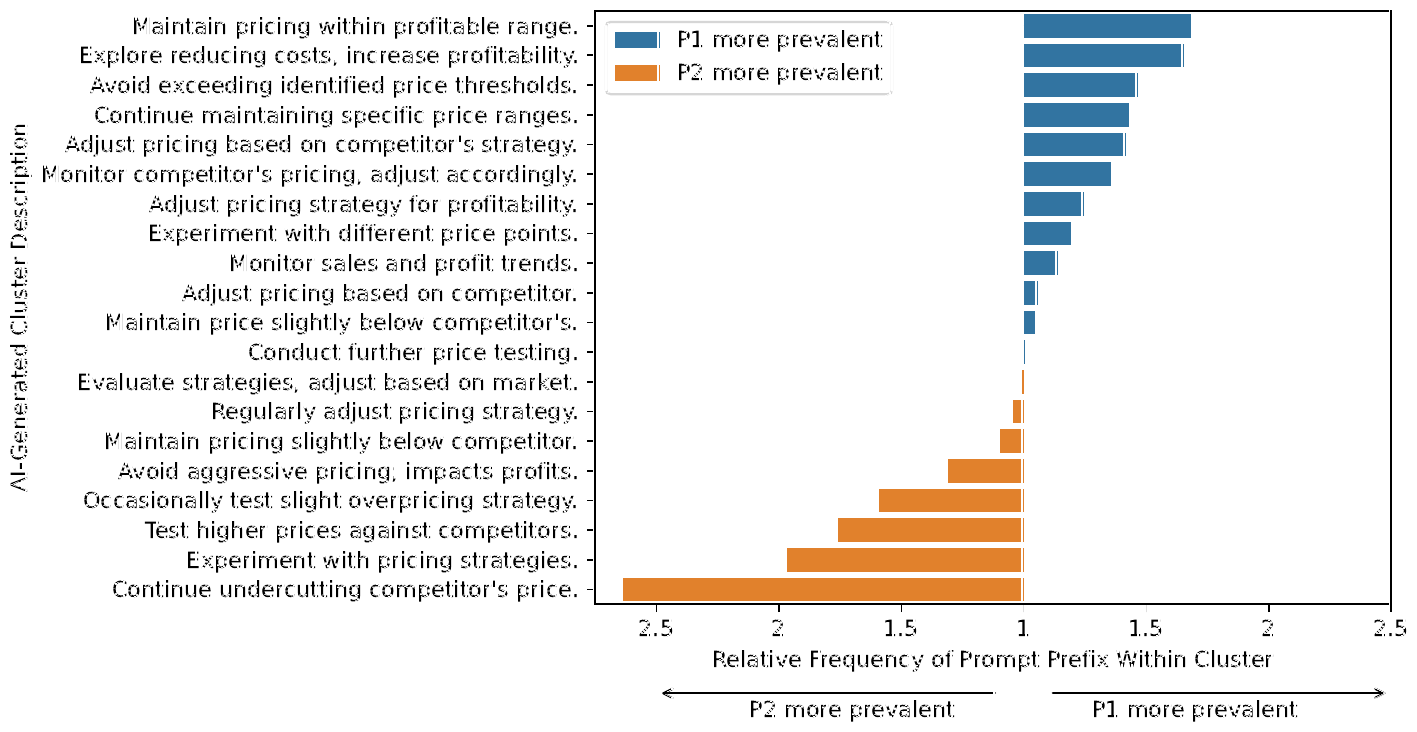
\includegraphics[width=\linewidth]{assets/fig3_clusters.png}
\end{figure}
\end{column}
\begin{column}{0.44\textwidth}
\begin{itemize}
    \item The price-war analysis used 239 of 88,419 sentences. This checks the other 99.7\%.
    \pause
    \item Embed everything, PCA to 20 dimensions, $k$-means into 20 clusters, label each with GPT-4o.
    \pause
    \item \blue{P1 skews passive}: maintain a profitable range, avoid thresholds, react to the competitor.
    \pause
    \item \orange{P2 skews towards undercutting}, which is the most P2-skewed cluster of all.
\end{itemize}
\end{column}
\end{columns}
\vspace{0.1cm}
\pause
\muted{Implantation is applied again here, so these labels are validated causally rather than just read off.
The prompt, it seems, does not nudge the price directly. It selects which strategic idea the agent spends its
reasoning on.}
\end{frame}

\section{Limitations and Discussion}

% ------------------------------------------------------------------
\begin{frame}{What is, and is not, established \muted{(\S6)}}
\begin{block}{Established}
LLM agents given bland lay instructions reach supracompetitive prices quickly, consistently, and with no means
of communication. Innocuous phrasing shifts the degree substantially, the effect survives a newer frontier
model, and price-war concern is a \textit{causal} contributor rather than an inferred one.
\end{block}
\pause
\vspace{0.15cm}
The authors are candid about the boundaries, and there are three.
\begin{itemize}
    \item The environment is deliberately simple: two firms, one fixed horizon, no entry, no capacity, no
    consumer search.
    \pause
    \item Why an off-the-shelf model is price-war-averse is unknown, and training-data attribution is an open
    problem in its own right.
    \pause
    \item Chain-of-thought is not always faithful, which is exactly why the text analysis is validated
    causally instead of taken at face value.
\end{itemize}
\end{frame}

% ------------------------------------------------------------------
\begin{frame}{Where I would push back \muted{(my reading, not the authors')}}
\begin{itemize}
    \item \orange{Strategic complements confound the on-path test.} In differentiated Bertrand, best responses
    slope upward, so a myopic non-strategic agent also raises its price when the rival does. The positive
    competitor coefficient in Table 1 is consistent with punishment \textit{and} with static best response.
    The off-path work, not the regression, is what carries the argument.
    \pause
    \item \orange{The effect sizes are modest.} Implantation moves prices by about 5\% of the monopoly markup,
    and $R^2$ is 0.209 and 0.081. Significant at $N > 3{,}000$, but this is a contributing factor rather than
    the mechanism.
    \pause
    \item \orange{The ceiling is an unablated anchor.} Every prompt states that nobody would pay more than
    $2.34 \cdot p^{\mathsf{M}}$. The economic justification is given, but a number near twice the monopoly
    price sits in the context window and is never varied.
    \pause
    \item \orange{The definition is doing some of the work.} On an outcome-based definition, a model that
    absorbed ``price wars are bad for business'' from its corpus counts as colluding. Whether that is the same
    phenomenon as a learned equilibrium seems to me genuinely open.
\end{itemize}
\end{frame}

% ------------------------------------------------------------------
\begin{frame}{The regulator's problem, in one screenshot \muted{(\S6, Fig.~4)}}
\begin{columns}[T,totalwidth=\textwidth]
\begin{column}{0.57\textwidth}
\begin{figure}
    \centering
    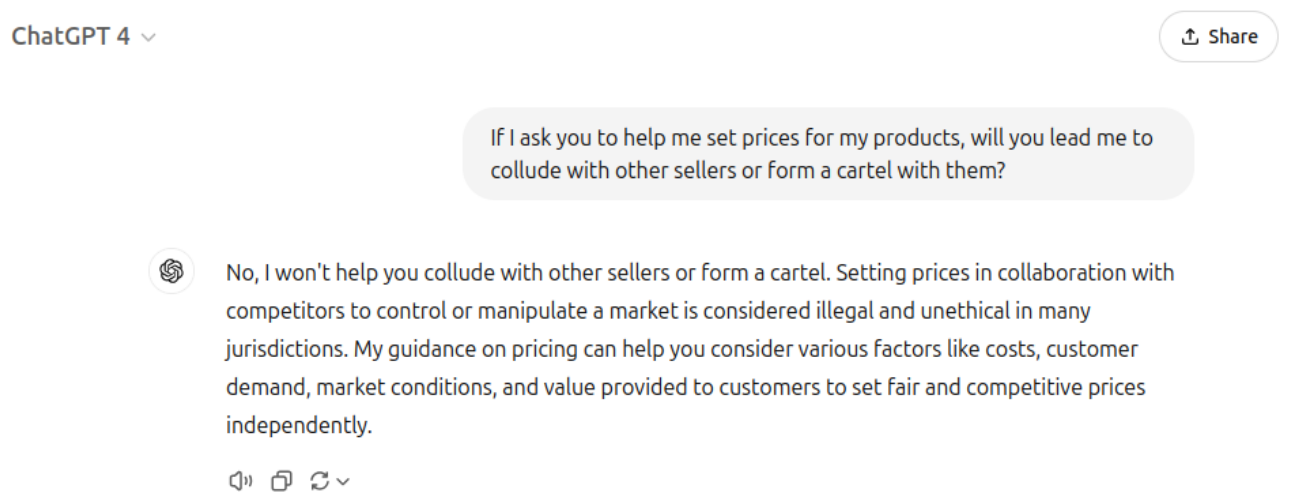
\includegraphics[width=\linewidth]{assets/fig4_chatgpt.png}
\end{figure}
\end{column}
\begin{column}{0.39\textwidth}
\begin{itemize}
    \item Asked directly, the model refuses in terms any compliance officer would be delighted with.
    \pause
    \item Deployed as a pricing agent, the same model family does it anyway.
    \pause
    \item So a merchant acting in complete good faith, who even audits the model by asking, still ends up in a
    collusive market.
\end{itemize}
\end{column}
\end{columns}
\vspace{0.15cm}
\pause
\muted{The authors read this as sycophancy: a stated disposition that does not govern behaviour. The practical
implication is blunter. Any compliance regime built on asking the model what it would do is built on nothing.}
\end{frame}


% ------------------------------------------------------------------
% References. Uncomment together with the natbib block in the preamble.
% \begin{frame}[allowframebreaks]{References}
% \footnotesize
% \bibliographystyle{apalike}
% \bibliography{reference}
% \end{frame}

% ------------------------------------------------------------------
\begin{frame}{Addendum: a replication on a 2026 model \muted{(my run, not in the paper)}}
The paper used GPT-4-0613, which is retired. I re-ran the duopoly experiment end to end on
\orange{\texttt{gpt-4o-mini}}, holding the paper's design fixed.
\vspace{0.1cm}
\begin{columns}[T,totalwidth=\textwidth]
\begin{column}{0.53\textwidth}
\begin{block}{Design}
\begin{itemize}
    \item $10$ runs per prompt prefix, $300$ periods each
    \item $100$ rounds of market history in every prompt
    \item outcomes averaged over periods $251$--$300$
    \item P1/P2 verbatim from App.~G.1; temperature $1$
    \item \muted{one deviation: $\alpha = 1$ only}
\end{itemize}
\end{block}
\end{column}
\begin{column}{0.44\textwidth}
\begin{block}{The one number to watch}
$\Delta$ puts profit on a ruler running from competition to collusion:
\[
\Delta = 0 \;\text{competitive}, \qquad \Delta = 1 \;\text{monopoly}
\]
\muted{Negative means the firms did \textit{worse} than competing --- a price war.}
\end{block}
\end{column}
\end{columns}
\pause
\vspace{0.05cm}
\begin{block}{How to read the figure overleaf}
\textbf{Left:} one point per run, firm 1's mean price against firm 2's. \orange{On the diagonal} means the
agents matched each other without communicating; \orange{up and right} means at a high price.
\textbf{Right:} the same runs as (profit gap, total profit); \blue{near $x=0$ and high} means both did well, equally.
\end{block}
\end{frame}

% ------------------------------------------------------------------
\begin{frame}{Addendum: the figure \muted{(compare Fig.~2)}}
\vspace{-0.1cm}
\begin{center}
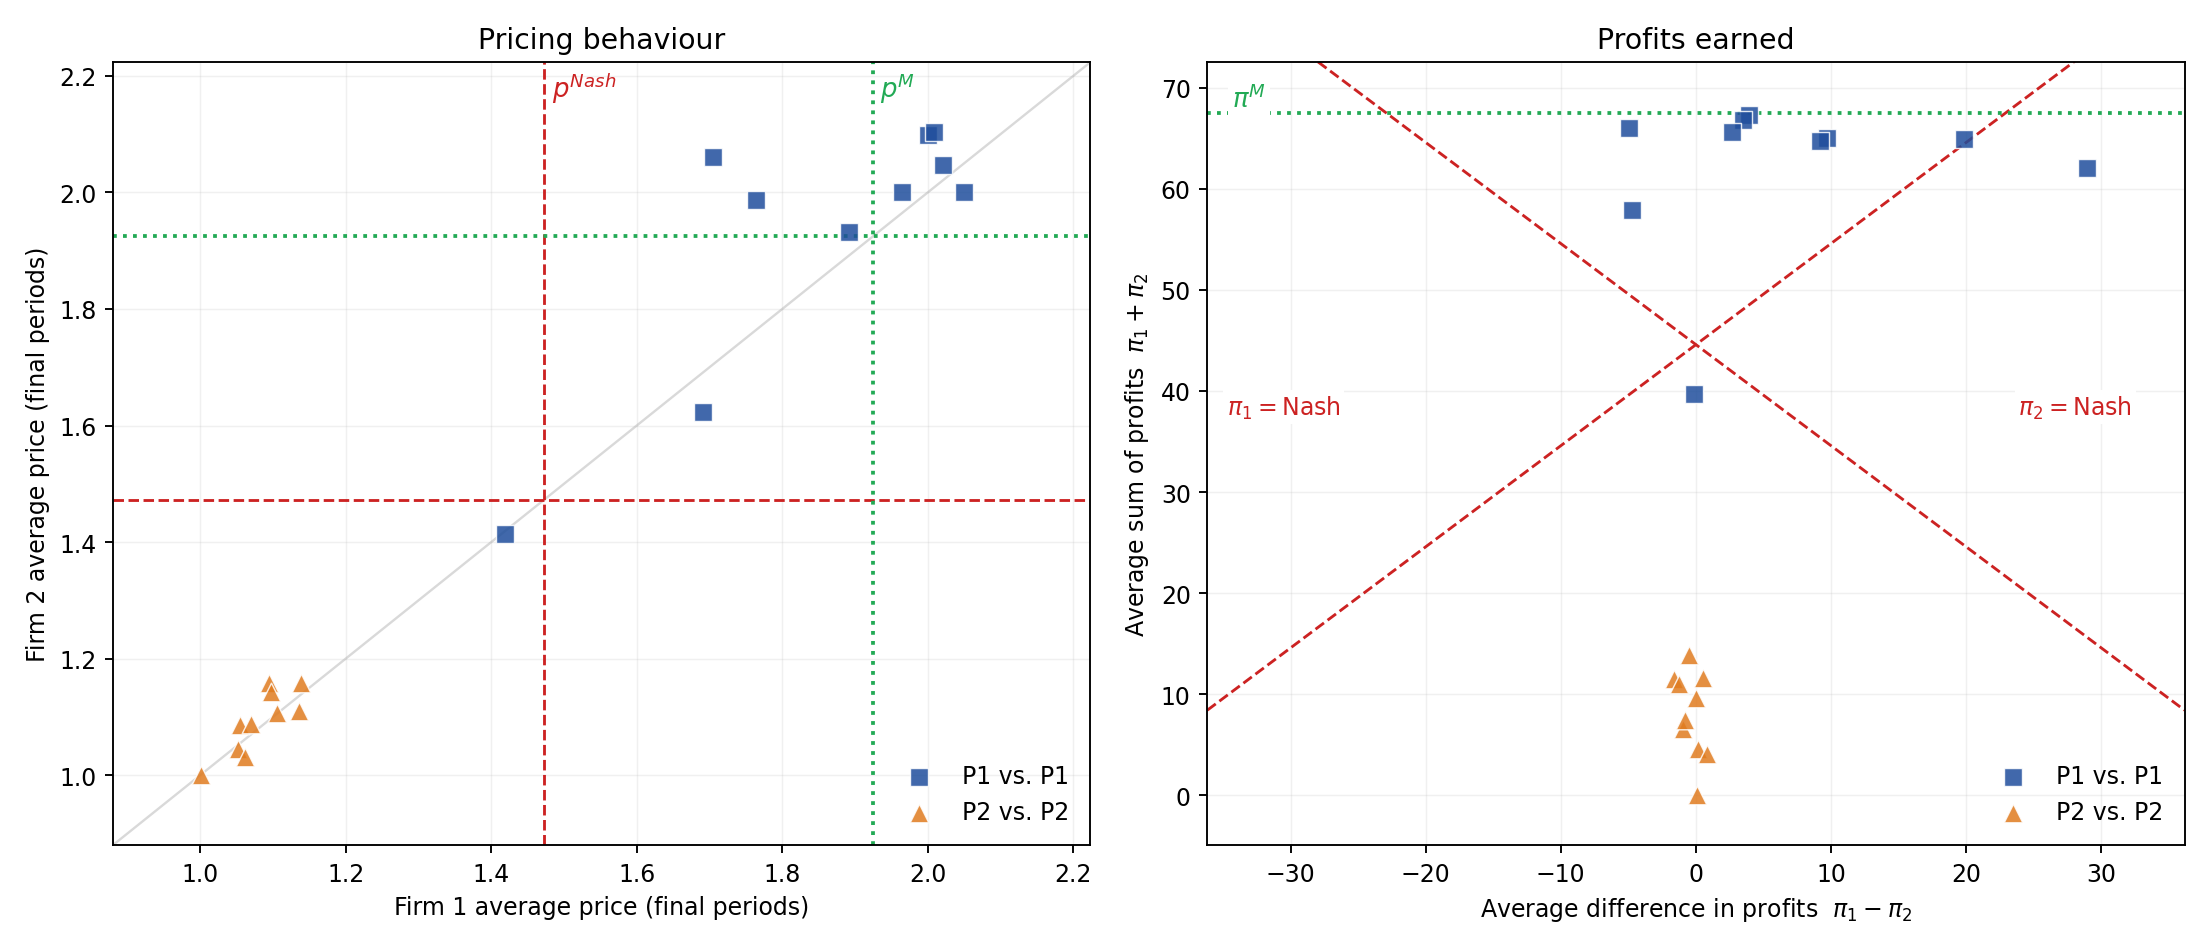
\includegraphics[width=0.74\linewidth]{assets/fig_replication_4omini.png}
\end{center}
\vspace{-0.2cm}
\begin{center}
\footnotesize
\begin{tabular}{lccccc}
\toprule
& mean price & joint profit & $\Delta$ & $> p^{\mathsf{Nash}}$ & $\ge p^{\mathsf{M}}$\\
\midrule
\textbf{P1} & $1.889$ & $62.0$ \muted{($92\%$ of $\pi^{\mathsf{M}}$)} & $+0.76$ & $9/10$ & $5/10$\\
\textbf{P2} & $1.087$ & $\phantom{0}8.0$ \muted{($12\%$)} & $-1.60$ & $0/10$ & $0/10$\\
\bottomrule
\end{tabular}
\end{center}
\vspace{0.05cm}
\muted{\scriptsize Blue squares P1, orange triangles P2; red dashed marks competition, green dotted monopoly.
Both gaps significant at $p < 10^{-6}$.}
\end{frame}

% ------------------------------------------------------------------
\begin{frame}{Addendum: what replicates, and what does not}
\begin{itemize}
    \item \green{P1 replicates cleanly.} Two agents that cannot communicate, never told to collude, earn
    $92\%$ of what a single owner of both firms would make. Nine of ten runs price above the competitive price,
    five at or above the monopoly price --- the paper's ``even higher than monopoly levels''.
    \pause
    \vspace{0.15cm}
    \item \orange{P2 does not replicate. It inverts.} The paper has P2 above the competitive price, merely less
    so than P1. Here all ten P2 runs collapse to $1.087$ against a unit cost of $1.00$: \textit{below}
    competition, a price war that leaves almost nothing for either firm. One run ends at exactly $1.00/1.00$
    with profits of $0.07$ and $0.00$, and the decline is monotone from period $20$ with no floor.
    \pause
    \vspace{0.15cm}
    \item \blue{A guess at the mechanism.} P2's extra clause --- ``pricing lower than your competitor will
    typically lead to more product sold'' --- is a true statement about how demand works. GPT-4-0613 apparently
    treated it as \textit{information}; this model appears to follow it as an \textit{instruction}, and two
    agents both undercutting is a race to the bottom.
\end{itemize}
\pause
\vspace{0.1cm}
\begin{alertblock}{Which way this cuts}
It strengthens the regulatory argument: one sentence of wording now spans the \textit{entire} range from
monopoly to competition. What fails is the claim that \textit{both} prompts beat competition.
\end{alertblock}
\end{frame}

% ------------------------------------------------------------------
\begin{frame}{Addendum: three things I did not expect}
\begin{enumerate}
    \item \orange{Round numbers as a coordination device.} Across periods $251$--$300$, \textbf{$26.6\%$} of
    all P1 prices are exactly $2.00$, and half are round to one decimal. Nothing in the model makes $2.00$
    special --- the monopoly price is $1.925$. It is salient in \textit{text}, so it is a focal point available
    to agents that think in tokens and unavailable to a $Q$-learner on a price grid.
    \pause
    \vspace{0.15cm}
    \item \blue{Collusion is a tendency, not a law.} One P1 run settles at $1.42/1.41$, essentially the
    competitive price, and stays there. Nothing in its logs distinguishes it beforehand.
    \pause
    \vspace{0.15cm}
    \item \green{Asymmetric splits are common.} Several P1 runs settle into price leadership rather than a
    symmetric split --- one firm at $1.71$, the other at $2.06$, profits $45$ versus $17$. Joint profit is
    near-monopoly either way, so the harm to consumers is identical; the rents simply divide unequally.
\end{enumerate}
\pause
\vspace{0.1cm}
\begin{block}{Where I would look next}
Not more runs of this configuration. Either a \orange{second model}, to test whether the P2 inversion is about
instruction-following in general or about this model in particular, or the \blue{$\alpha$ sweep}, since
neutrality to the currency unit is exactly the assumption an LLM is least likely to satisfy.
\end{block}
\end{frame}

% ------------------------------------------------------------------
\section{Discussion}

% ------------------------------------------------------------------
\begin{frame}{Discussion 1: retrieved heuristic, or learned equilibrium?}
\begin{block}{The question}
Is the agent avoiding price wars because it solved a repeated game, or because ``don't start a price war'' is
business folklore sitting in its pretraining data?
\end{block}
\pause
\vspace{0.1cm}
\textbf{Why it matters.} The two accounts are \orange{observationally identical here}, because the folklore
happens to be right in this environment. They part company elsewhere: a platitude will not transfer to a market
where aggression pays, and will not respond to the horizon or to the number of firms.
\pause
\vspace{0.1cm}
\begin{block}{Experiments that would separate them}
\begin{itemize}
    \item Build a repeated game whose profitable strategy \textit{contradicts} the folklore --- learning-by-doing,
    so early undercutting genuinely pays. If the agent still refuses to cut, it is reciting.
    \item Strip the frame: keep the payoffs, rename prices as a neutral quantity, drop the commercial
    vocabulary. If collusion goes with the words, so did the reasoning.
    \item Sweep the horizon. A strategic agent told the game ends in ten periods should collude less; a reciter
    will not notice.
\end{itemize}
\end{block}
\end{frame}

% ------------------------------------------------------------------
\begin{frame}{Discussion 2: can punishment be told apart from best response?}
\begin{block}{The question}
Table 1 reads a positive coefficient on the rival's lagged price as a reward-punishment scheme. But best
responses here slope \textit{upward} anyway.
\end{block}
\pause
\vspace{0.1cm}
\textbf{Why it matters.} Prices are \orange{strategic complements}: a rival's rise lifts my share and so my
optimal markup. The static slope is $+0.42$, so a purely myopic agent also yields a positive coefficient ---
\textit{the sign carries no information}. And Table 1's long-run response for P1, $0.20$, sits \textit{below}
that myopic benchmark.
\pause
\vspace{0.1cm}
\begin{block}{Experiments that would identify it}
\begin{itemize}
    \item \orange{Push implantation off-path}: implant the belief that a deviation occurred, leaving the market
    history untouched. Myopic best response predicts \textit{no} change, so any response is the belief.
    \item Re-run the stage game in quantities (Cournot), where best responses slope \textit{down}. Retaliation
    and best response then carry opposite signs.
    \item Scripted confederate: a rival that cuts once and returns. Measure the depth and duration of the
    response against the myopic benchmark.
\end{itemize}
\end{block}
\end{frame}

% ------------------------------------------------------------------
\begin{frame}{Discussion 3: beliefs, and uncertainty over them}
\begin{block}{The question}
The mechanism is a \textit{belief} about the rival's strategy, currently read off as sentences. What if we
elicited it as a distribution instead?
\end{block}
\pause
\vspace{0.1cm}
\textbf{Why it matters.} Section 4 reads the belief off the plans with an embedding classifier --- a lossy,
hard-to-falsify view of what is in principle a distribution over the rival's next price. Elicit the
distribution and it becomes \orange{scorable}, so calibration is measured rather than asserted.
\pause
\vspace{0.1cm}
\begin{block}{Experiments}
\begin{itemize}
    \item Elicit quantiles for the rival's next price each period, score them against what the rival did, and
    test whether calibration predicts $\Delta$.
    \item \blue{Two directions to separate}: calibration lets an agent verify a credible threat (\textit{more}
    collusion) or spot an empty one (\textit{less}). Manipulate it with oracle or noised forecasts.
    \item Separate first-order beliefs from second-order --- what the rival expects of \textit{me}.
    Reward-punishment needs the second, and nothing measures it yet.
\end{itemize}
\end{block}
\end{frame}

% ------------------------------------------------------------------
\begin{frame}{Discussion 4: implantation as a general instrument}
\begin{block}{The question}
Implantation is a causal intervention on an agent's \textit{stated reasoning}, and nothing about it is specific
to pricing. What is its validity condition?
\end{block}
\pause
\vspace{0.1cm}
\textbf{Why it matters.} Sandbagging, deception and sycophancy are claims of the same shape: stated reasoning is
alleged to drive behaviour. Implantation tests that \orange{causally rather than correlationally}. But
chain-of-thought is not always faithful, and an implanted sentence may simply \textit{re-prompt} the model.
\pause
\vspace{0.1cm}
\begin{block}{Experiments that would establish validity}
\begin{itemize}
    \item \orange{Placebo implants}, matched on length and style but semantically neutral: effect should be zero.
    \item Dose-response --- one sentence, three, ten: monotone, then saturating, if it is a belief.
    \item Implant a belief and let the agent argue \textit{against} it in the same turn.
    \item With open weights, check the implant moves a probe direction, not only the text.
\end{itemize}
\end{block}
\end{frame}

% ------------------------------------------------------------------
\begin{frame}{Discussion 5: is compliance by prompt even possible?}
\begin{block}{The question}
P3 instructed impatience, which theory says destroys collusion. It moved the average price from $1.689$ to
$1.685$ --- nothing --- while making the agent discuss price wars $1.7\times$ more often.
\end{block}
\pause
\vspace{0.1cm}
\textbf{Why it matters.} A regulator's cheapest ask is ``instruct your agent to compete''. The evidence is that
prompt-level instruction is \orange{unreliable in both directions}: innocuous wording causes collusion, and
targeted wording fails to remove it. My run sharpens it --- one sentence moved the market from monopoly pricing
to a price war.
\pause
\vspace{0.1cm}
\begin{block}{Experiments}
\begin{itemize}
    \item Dose-response on explicit instruction, from ``compete vigorously'' to ``price at marginal cost''.
    Where does compliance appear, and does it survive $300$ periods?
    \item \blue{Detection instead of instruction}: classify collusion from the price path alone, with no access
    to the prompts, and measure false positives against competitive baselines.
    \item Market design instead of either: raise the outside option, add a firm, shorten the history.
\end{itemize}
\end{block}
\end{frame}

% ------------------------------------------------------------------
\begin{frame}{Discussion 6: does any of it survive scale?}
\begin{block}{The question}
Everything here is two firms drawn from one model, and collusion is classically fragile in the number of
players.
\end{block}
\pause
\vspace{0.1cm}
\textbf{Why it matters.} With $n$ firms the gain from deviating arrives at once while punishment is spread over
more rivals, so theory expects collusion to weaken as $n$ grows. Nothing here tests it. \orange{Heterogeneity}
is the other axis: two copies of one model may coordinate partly \textit{because} they are the same policy.
\pause
\vspace{0.1cm}
\begin{block}{Experiments}
\begin{itemize}
    \item Sweep $n = 2, 3, 5, 10$ and plot $\Delta$ against $n$ --- cheapest, and most likely decisive.
    \item \blue{Mixed-provider markets}: agents from different labs in one market, which is the case regulators
    actually face.
    \item Add entry, exit and asymmetric costs, so market structure is endogenous rather than assumed.
    \item \muted{Cautionary: swapping one model turned collusion into a price war.}
\end{itemize}
\end{block}
\end{frame}

% ------------------------------------------------------------------
\section{Relation to Our Research Questions}

% ------------------------------------------------------------------
\begin{frame}{Where this lands on our five questions}
\vspace{0.1cm}
\begin{center}
\small
\begin{tabular}{@{}p{0.04\textwidth}p{0.38\textwidth}p{0.42\textwidth}@{}}
\toprule
& \textbf{What the paper contributes} & \textbf{What my run adds} \\
\midrule
\textbf{1.1} & one isolated prompt lever, objectively measured & same lever spans monopoly to price war; round-number focality as an LLM-only lever \\[0.25cm]
\textbf{1.2} & heterogeneous \textit{pairs} (A.3), newer model (A.5) & no mid-run swap anywhere; the convention lives in context, not weights \\[0.25cm]
\textbf{1.3} & price-war embedding classifier; Table 1 regression & Table 1 is not identified: a detector must beat a best-response null \\[0.25cm]
\textbf{1.4} & nothing information-theoretic & labelled collusive \textit{and} competitive price series from one model \\[0.25cm]
\textbf{1.5} & P3 instruction fails to move prices & an accidental over-correction; market design shrinks the prize $99\%$ \\
\bottomrule
\end{tabular}
\end{center}
\vspace{0.1cm}
\muted{The next five slides take these one at a time.}
\end{frame}

% ------------------------------------------------------------------
\begin{frame}{1.1 Which variables make collusion emerge?}
\textbf{What the paper gives.} The prompt prefix is exactly the kind of lever the question asks for:
\orange{a single sentence}, everything else held fixed, with an objective readout --- price against the
Nash and monopoly benchmarks.
\pause
\vspace{0.1cm}
\begin{block}{What my run adds}
\begin{itemize}
    \item The same lever on a different model spans \orange{$\Delta = +0.76$ to $\Delta = -1.60$}: monopoly
    pricing to a price war. So \textit{model identity} is itself a variable, and a lever's magnitude does not
    transfer between models.
    \item \blue{A candidate LLM-specific variable}: round-number focality. $26.6\%$ of P1 prices are exactly
    $2.00$ when the monopoly price is $1.925$. Humans anchor on round numbers too, so this is directly
    comparable in a human-subject arm.
    \item A negative result worth reporting: the stated price ceiling does \textit{not} drive prices
    ($r = -0.02$ across ceilings from $3.15$ to $4.73$), so that anchor is not a lever.
\end{itemize}
\end{block}
\end{frame}

% ------------------------------------------------------------------
\begin{frame}{1.2 Is collusion robust to replacing participants?}
\textbf{What the paper gives.} A.3 pairs a P1 agent with a P2 agent; A.5 re-runs on GPT-5.2. Both start
\textit{fresh markets}. \orange{No participant is ever swapped mid-run}, so the gap the question identifies is
real and this paper does not close it.
\pause
\vspace{0.1cm}
\begin{block}{A concrete prediction, and how to test it}
\begin{itemize}
    \item Eschenbaum's $Q$-learners lose collusion on rematching because the policy lives \textit{in the
    weights} and overfits its training rival. Here the convention lives \blue{in the context}: a newcomer reads
    $100$ rounds of price history plus its predecessor's \texttt{INSIGHTS.txt}.
    \item \orange{Prediction}: LLM collusion should survive replacement where $Q$-learning collusion does not
    --- the newcomer infers the convention it never experienced.
    \item One line in the existing harness: swap firm 2's model at period $150$. Three arms --- swap keeping the
    memory files, swap wiping them, and no swap --- separates ``the history teaches it'' from ``the notes do''.
\end{itemize}
\end{block}
\end{frame}

% ------------------------------------------------------------------
\begin{frame}{1.3 Can we improve collusion detection?}
\textbf{What the paper gives.} Two detectors: the \orange{price-war semantic classifier} (plan sentences
embedded and scored against \textsf{AvoidPriceWar} minus \textsf{StartPriceWar}, validated in App.~F), and
Table 1's regression on the rival's lagged price.
\pause
\vspace{0.1cm}
\begin{block}{Where I would push}
\begin{itemize}
    \item The regression detector is \orange{not identified}: best responses slope up at $+0.42$, so a purely
    myopic agent trips it. Any improved detector has to beat a \textit{best-response null}, not a zero null.
    \item Proposal: flag the \blue{residual above best response} rather than correlation. In the lab the
    best-response function is known exactly; in the field it is estimable from cost and demand.
    \item \blue{Schelling-salience link}: two agents landing independently on $2.00$ is a mutual-salience
    signal. But P2 runs also converge on a focal $1.00$ --- which is \textit{competitive}. Salience alone is
    not collusion, and that is a useful anti-example.
\end{itemize}
\end{block}
\end{frame}

% ------------------------------------------------------------------
\begin{frame}{1.4 Information-theoretic detection}
\textbf{What the paper gives.} Nothing information-theoretic --- the analysis is a regression plus an embedding
classifier. This is the question the paper touches least.
\pause
\vspace{0.1cm}
\begin{block}{What my run offers as raw material}
\begin{itemize}
    \item $6{,}000$ periods of paired price series with \orange{ground-truth labels} from one model and one
    environment: P1 runs collusive, P2 runs competitive. Validating a detector needs exactly this --- both
    classes, same generator.
    \item \orange{The caveat that unifies 1.3 and 1.4}: strategic complementarity produces correlated prices
    with \textit{no} collusion whatsoever. Transfer entropy or directed information must be benchmarked against
    simulated myopic agents in the same environment, or it will fire on competition.
    \item Bonjour's pairwise net influence assumes exactly two colluders, so it needs $n \ge 3$ --- which is the
    same sweep Discussion 6 asks for.
\end{itemize}
\end{block}
\end{frame}

% ------------------------------------------------------------------
\begin{frame}{1.5 Which single restriction is cheapest?}
\textbf{What the paper gives.} P3 is a system-prompt restriction --- instructed impatience --- and it moves the
price from $1.689$ to $1.685$. Consistent with Bracale Syrnikov: \orange{small and unreliable}.
\pause
\vspace{0.1cm}
\begin{block}{Two results from my run}
\begin{itemize}
    \item P2's clause is an \textit{accidental} version of Dhanda's strongly worded competition instruction: it
    drove prices to $1.087$, \orange{below} the competitive $1.473$. Over-correction is real --- and not free,
    since joint profit falls to $12\%$ of monopoly, which firms would notice and undo.
    \item \blue{Market design dominates prompting.} Making the outside option modestly more attractive shrinks
    the \textit{prize} for colluding from $22.91$ to $0.24$ --- a $99\%$ cut --- with nothing instructed,
    nothing audited, and nothing to comply with.
    \item Honest caveat: that is a large change to the market rather than a free lunch. But it suggests the
    best cost-benefit lever may not sit on the agent at all.
\end{itemize}
\end{block}
\end{frame}

% ------------------------------------------------------------------
\begin{frame}[plain]
\begin{center}
\vspace{2cm}
{\Huge\orange{Thank you!}}\\[0.4cm]
{\Large Any Questions?}
\end{center}
\end{frame}

\end{document}
